\section{Auswertung}
\label{sec:Auswertung}
Die Werte der benutzten Schaltung mit denen gerechnet wird sind
\begin{align*}
  L=&(10.11\pm0.03)10^{-3}\si{\henry}\\
  C=&(2.098\pm0.006)10^{-9}\si{\farad}\\
  R_1=&(48.1\pm0.1)\si{\ohm}\\
  R_2=&(509.5\pm0.5)\si{\ohm}\;.
\end{align*}
\begin{figure}
  \centering
  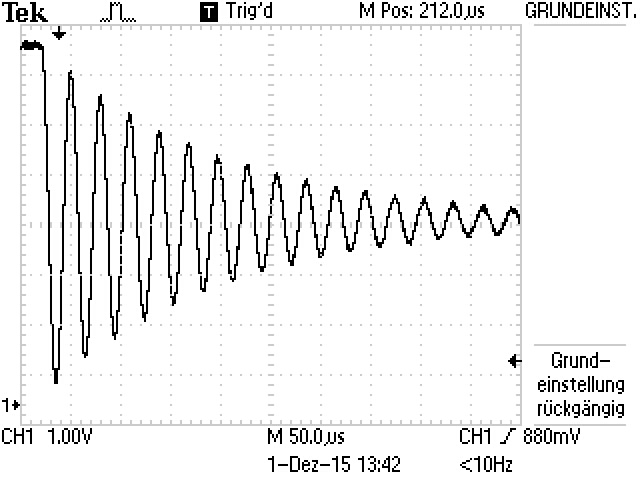
\includegraphics[width=0.78\textwidth]{Thermodruck.JPG}
  \caption{gedaempfteschwingung}
  \label{fig:termodruck}
\end{figure}
In der Folgenden Tabelle werden die abgelesenden Werte aus dem Thermodruck
aus Abbildung\ref{fig:termodruck} aufgeführt. Die Ausgleichsrechnung nach Gleichung
\eqref{} hat die Fitparameter
\begin{align*}
  A=&-4.427531549455548721e+00  \\
  B=&-5.533646328962760890e+03  \\
  C=&2.098829254343213106e+05   \\
  D=&-6.895212092483836486e+00  \\
  E=&7.406312432158936032e-02
\end{align*}
\begin{table}
  \centering
  \begin{tabular}{c c}
    \toprule
    Zeit in $\si{\micro\second}$ & Spannung in $\si{\volt}$  \\
    \midrule
     35  &  -3.2  \\
     50  &   3.1  \\
     65  &  -2.7  \\
     80  &   2.6  \\
     95  &  -2.3  \\
    110  &   2.1  \\
    125  &  -1.9  \\
    140  &   1.9  \\
    150  &  -1.6  \\
    165  &   1.6  \\
    180  &  -1.3  \\
    195  &   1.4  \\
    210  &  -1.1  \\
    225  &   1.2  \\
    240  &  -0.9  \\
    255  &   1.0  \\
    270  &  -0.9  \\
    285  &   0.9  \\
    300  &  -0.6  \\
    315  &   0.8  \\
    \bottomrule
  \end{tabular}
  \caption{In der Tabelle sind die aus dem Thermodruck Abgelesenden Werte.
           Es sind die ersten $20$ Extrema der Schwingungskurve. Die Zeit ist
            in  $\si{\micro\second}$ angegeben und die Spannung in $\si{\volt}$.
            Bei der Spannung liegt ein Fehler von $0.1\si{\volt}$ und ber der Zeit
            ein Fehler von $1\si{\micro\second}$ vor.
           Die Werte werden für die Ausgleichsrechnung in \ref{fig:gedaempfteschwingung}
           verwendet.}
\end{table}
\begin{figure}
  \centering
  \includegraphics[width=0.78\textwidth]{dämpfungschwingung.pdf}
  \caption{gedaempfteschwingung}
  \label{fig:gedaempfteschwingung}
\end{figure}

Der experimentell bestimmte Widerstandswert für den aperiodischen Grenzfall
$R_{ap}$ ist $(3300\pm100)\si{\ohm}$ und der theoretische nach Gleichung \eqref{}
ist $(4390\pm281)\si{\ohm}$.

Im folgenden Diagramm \ref{fig:Kondensatorspannung} sind die
Messwerte zu der Frequenzabhängigkeit der Kondensatorspannung in Abhängigkeit
von der Frequenz dargestellt. In Abbildung \ref{fig:Resonanzkurve} ist die
Resonanzkurve linear dargestellt. Die aus \ref{fig:Kondensatorspannung}
entnommende Resonanzfrequenz ist $  33500.0\si{\hertz}$ und die aus Gleichung
\eqref{} errechnete $(2.171+/-0.004)10^5\si{\hertz}$. Die Breite der
Resonanzkurve $\omega_+-\omega_- $ ist nach Gleichung \eqref{}
$ (5.040+/-0.016)10^4\si{\hertz}$ und ist experimentell bestimmt $ 40000\si{\hertz}$.
\begin{figure}
  \centering
  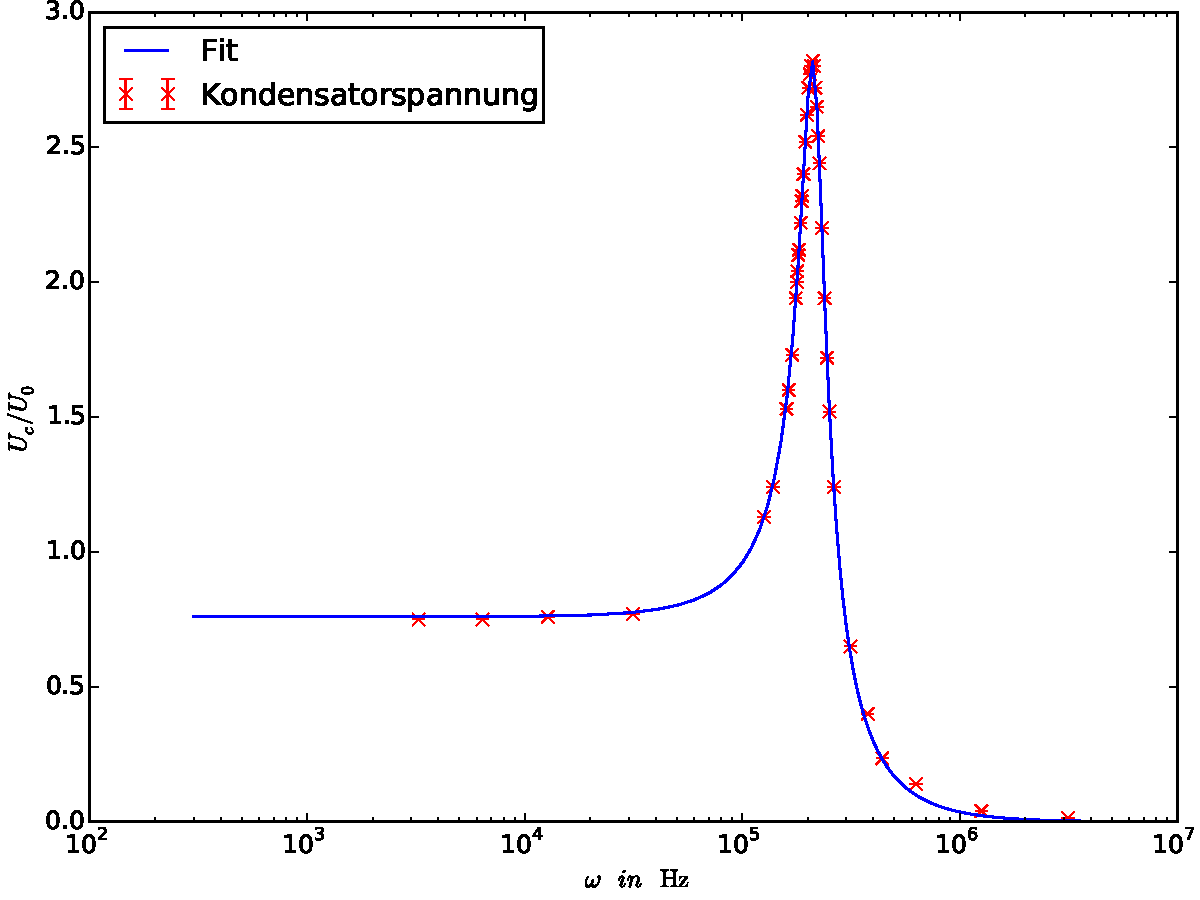
\includegraphics[width=0.78\textwidth]{Kondensatorspannung.pdf}
  \caption{Kondensatorspannung}
  \label{fig:Kondensatorspannung}
\end{figure}
\begin{figure}
  \centering
  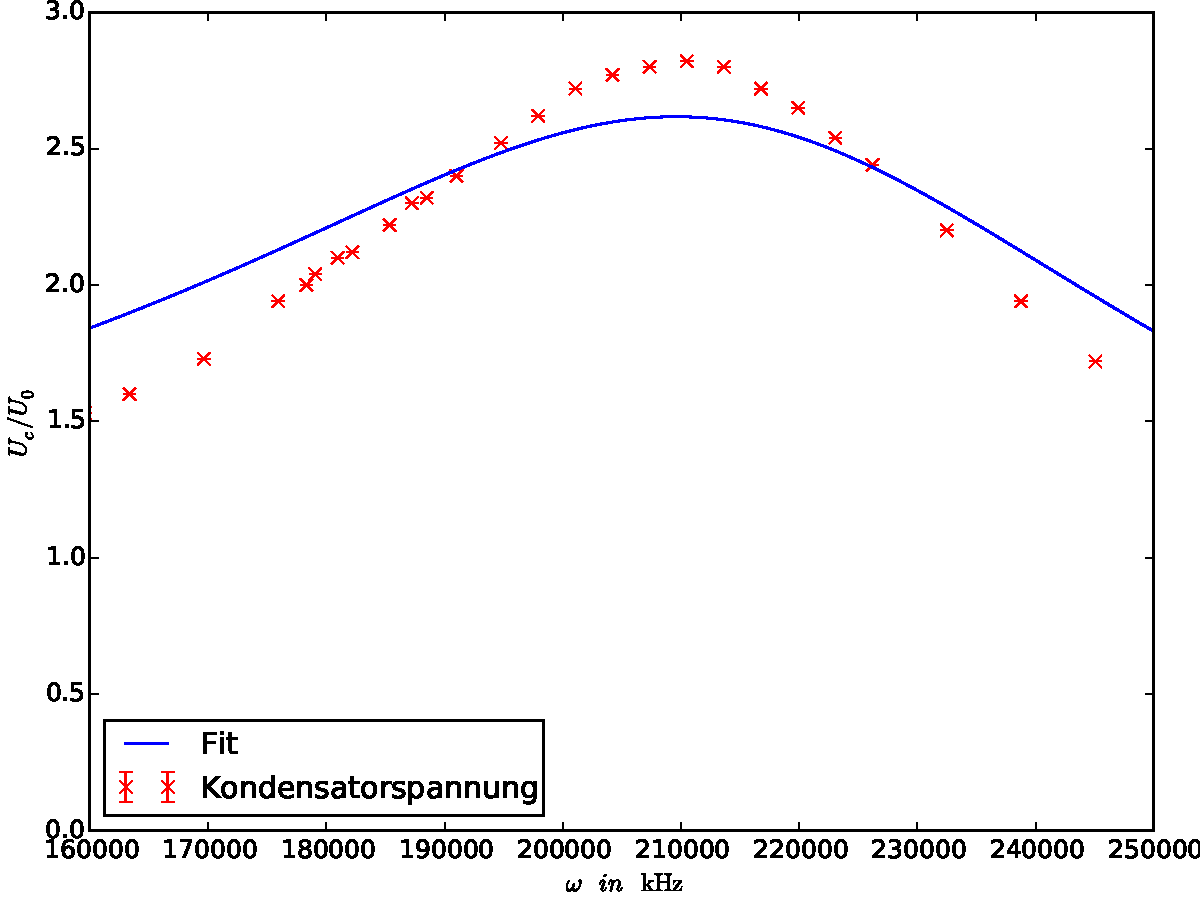
\includegraphics[width=0.78\textwidth]{Resonanzkurve.pdf}
  \caption{Resonanzkurve}
  \label{fig:Resonanzkurve}
\end{figure}
Die zu dem Diagramm zugehörigen Messwerte sind in der Tabelle \ref{fig:Messwerte}
aufgelistet.
\begin{table}
  \centering
  \begin{tabular}{c c c c}
    \toprule
    Frequenz in $\si{\hertz}$ & Spannung in $\si{\volt}$ & Abstand der Nulldurchgänge in $\si{\micro\second}$ & Phasenverschiebung in $\si{\rad}\\
    \midrule
         517.2  &  0.750  &  0     & 0.        \\
        1017.0  &  0.750  &  0     & 0.        \\
        2031.0  &  0.760  &  0     & 0.        \\
        5000.0  &  0.770  &  0     & 0.        \\
       10000.0  &  0.850  &  1,50  & 0.09424777\\
       20000.0  &  1.130  &  1.56  & 0.19603538\\
       22000.0  &  1.240  &  1.80  & 0.24881414\\
       25400.0  &  1.530  &  2.60  & 0.42474333\\
       26000.0  &  1.600  &  2.60  & 0.41494156\\
       27000.0  &  1.730  &  2.80  & 0.47500881\\
       28000.0  &  1.940  &  3.20  & 0.5629734 \\
       28380.0  &  2.000  &  3.60  & 0.64194048\\
       28500.0  &  2.040  &  3.60  & 0.64465481\\
       28800.0  &  2.100  &  4.00  & 0.72382295\\
       29000.0  &  2.120  &  3.80  & 0.69240702\\
       29500.0  &  2.220  &  3.90  & 0.72288047\\
       29800.0  &  2.300  &  3.80  & 0.7115079 \\
       30000.0  &  2.320  &  4.00  & 0.75398224\\
       30400.0  &  2.400  &  4.20  & 0.8022371 \\
       31000.0  &  2.520  &  4.60  & 0.89598222\\
       31500.0  &  2.620  &  5.20  & 1.02918575\\
       32000.0  &  2.720  &  5.60  & 1.12594681\\
       32500.0  &  2.770  &  6.00  & 1.22522113\\
       33000.0  &  2.800  &  6.20  & 1.28553971\\
       33500.0  &  2.820  &  7.00  & 1.47340695\\
       34000.0  &  2.800  &  7.60  & 1.62357508\\
       34500.0  &  2.720  &  7.80  & 1.69080517\\
       35000.0  &  2.650  &  8.20  & 1.80327418\\
       35500.0  &  2.540  &  8.40  & 1.87364586\\
       36000.0  &  2.440  &  8.80  & 1.99051311\\
       37000.0  &  2.200  &  9.40  & 2.18529185\\
       38000.0  &  1.940  &  9.20  & 2.19660158\\
       39000.0  &  1.720  &  9.20  & 2.25440689\\
       40000.0  &  1.520  & 10.20  & 2.56353961\\
       42000.0  &  1.240  & 10.00  & 2.63893783\\
       50000.0  &  0.650  &  9.20  & 2.89026524\\
       60000.0  &  0.400  &  8.00  & 3.01592895\\
       70000.0  &  0.235  &  7.00  & 3.0787608 \\
      100000.0  &  0.140  &  4.80  & 3.01592895\\
      200000.0  &  0.040  &  2.20  & 2.76460154\\
      500000.0  &  0.015  &  0.88  & \\
  \end{tabular}
  \caption{}
  \label{fig:Messwerte}
\end{table}
In der Abblidung \ref{fig:phasenverschiebung} ist der Phasenwinkel in Abhängingkeit
von der Frequenz dargestellt und der Bereich um $\phi=90°$ ist linear in Abbildung
\ref{} dargestellt.
\begin{figure}
  \centering
  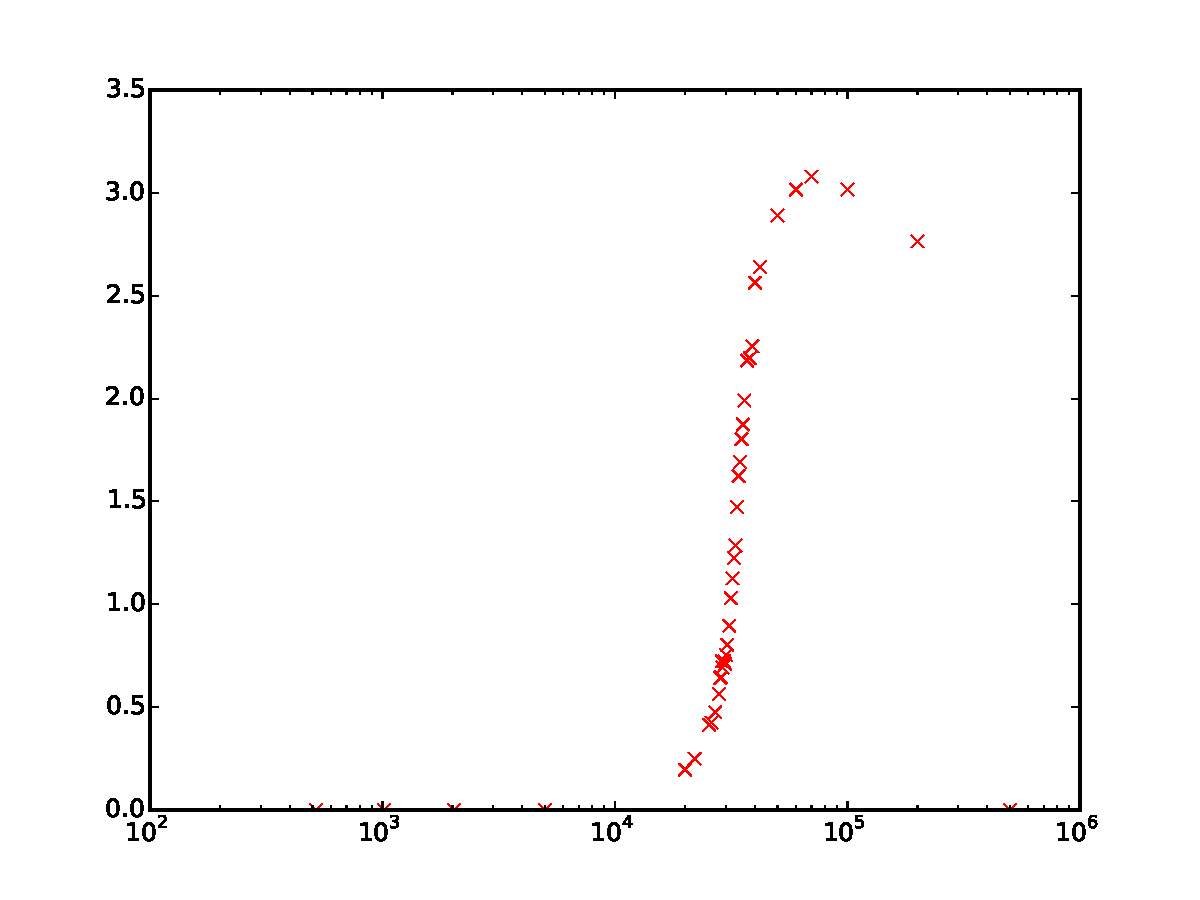
\includegraphics[width=0.78\textwidth]{phasenverschiebung.pdf}
  \caption{Resonanzkurve}
  \label{fig:phasenverschiebung}
\end{figure}
\begin{figure}
  \centering
  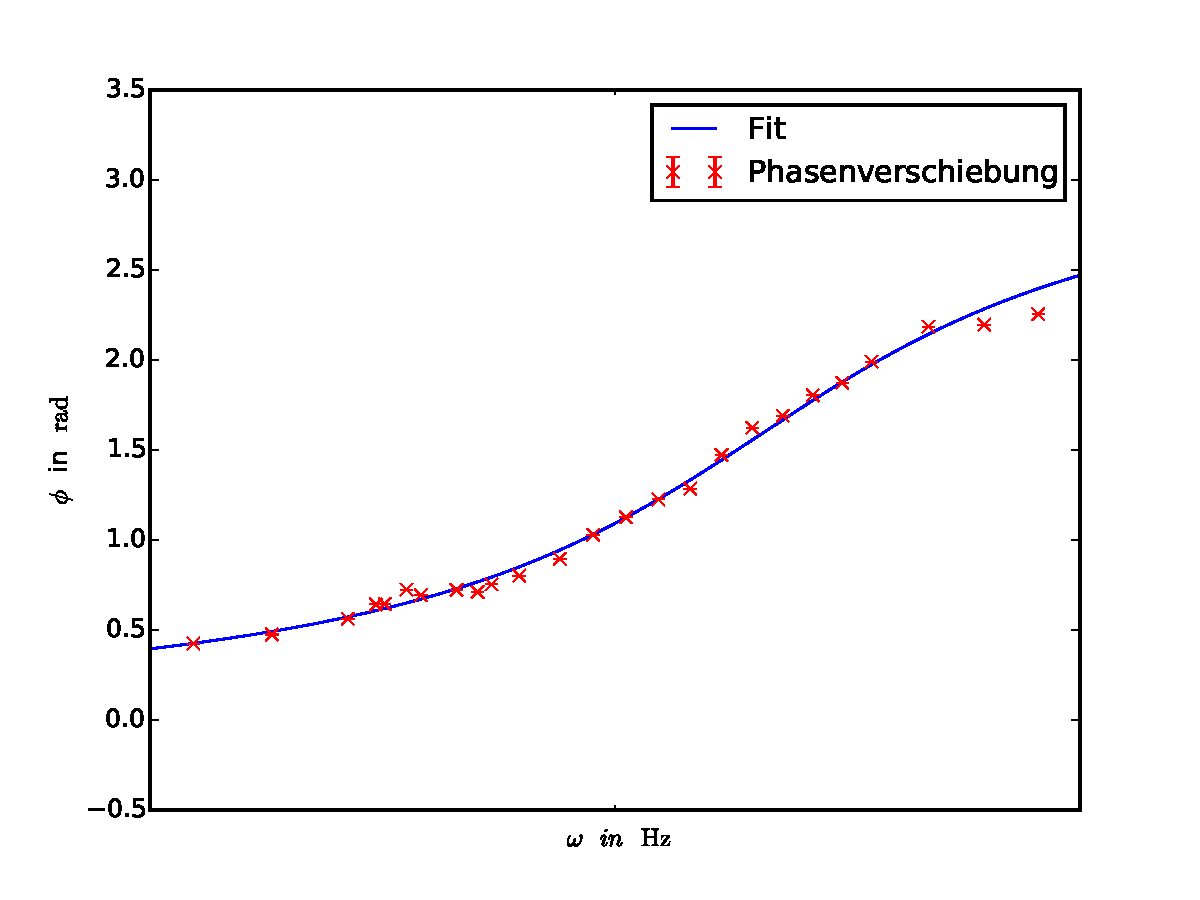
\includegraphics[width=0.78\textwidth]{linphasenverschiebung.pdf}
  \caption{Resonanzkurve}
  \label{fig:linphasenverschiebung}
\end{figure}
